\section{2つの球のヘルツ接触}
ここでは、Code\_Asterのベンチマーク問題SSNV104を例に説明します。
この例では、接触している2つの球体が互いに押し付けられています。
対称性を利用して、それぞれの球体の1/8だけを分析する必要があります。
\vskip.5\baselineskip
ジオメトリは、CADソフトウェアで個別のパーツとしてモデル化され、そのアセンブリをステップ形式でインポートする必要があります。
\begin{enumerate}
\item
  {[}mm, ton, s, °C{]}単位の新規ファイルを作成し、ステップ形式のジオメトリをPrePoMaxにインポートします。
  次に、両方のパーツをメッシュ分割します。
  ここでは、最大要素サイズとして5mmを選択し、その他の設定は変更しませんでした。
  さらに、接触領域に0.5mmの局所的なメッシュ細分化を適用しました(メッシュをより良く細分化するには、球体を分割して、細分化を割り当てることができるエッジを作成する必要があります)。
  そうしないと、ユーザーは接触点の頂点を使用しなければなりません(図\ref{fig:08-01})。
	\begin{figure}[H]
	\centering
	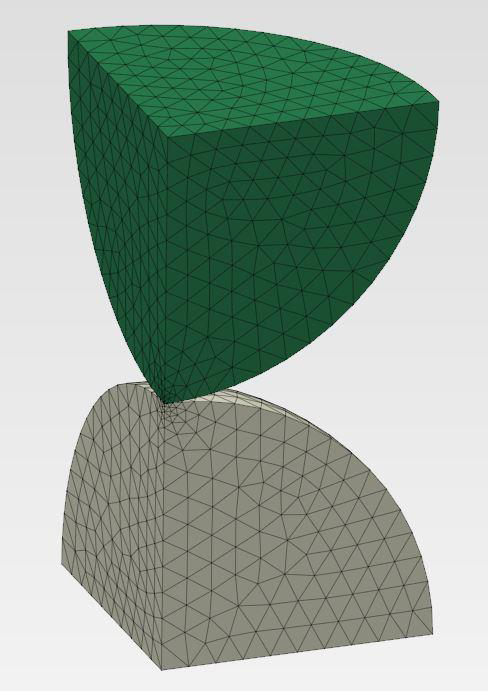
\includegraphics[width=67mm]{fig/08-01.png}
	\caption{2つの球 - メッシュ}
	\label{fig:08-01}
	\end{figure}
\item
  新しい材料を定義し、弾性挙動を加え、ヤング率を20000MPa、ポアソン比を0.3と指定します。
  先に作成した材料を参照して新しいソリッドセクションを作成し、そのセクションがこのパーツに割り当てられるように両方の球セグメントを選択します。
\item
  デフォルトのサーフェス挙動(ハード)でサーフェスの相互作用を作成します。
  この相互作用を参照してコンタクトペアを作成し、解析中に接触する2つのサーフェスを選択します。
\item
  新しい静的ステップを作成し、Nlgeomをオンにします(幾何学的非線形性を考慮するため)。
  2つの変位/回転境界条件を定義し、対称性のある2つの側面からなる2つのセットに適用します(各セットの面の法線方向の変位のみを拘束します)。
  さらに2つの変位/回転境界条件を作成し、上面と下面に割り当てます。
  矢印が互いに向き合い、球が互いに押し付けられるように、2mmと-2mmの変位を規定します(図\ref{fig/08-02.png})。
	\begin{figure}[H]
	\centering
	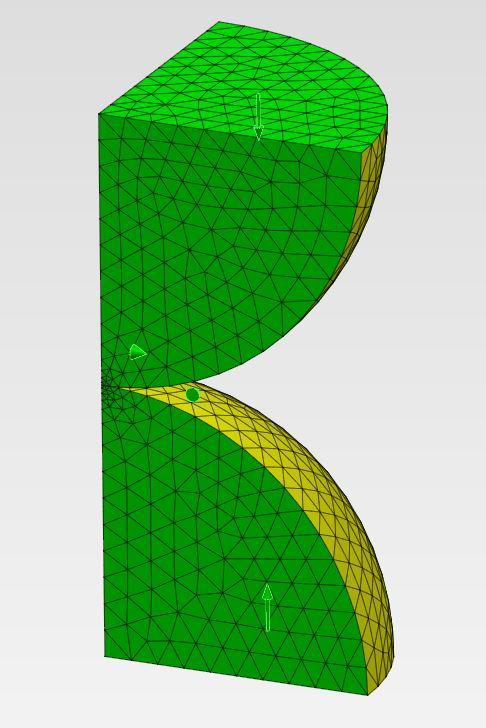
\includegraphics[width=67mm]{fig/08-02.png}
	\caption{2つの球 - 境界条件}
	\label{fig:08-02}
	\end{figure}
\item
  解析を実行し、解析が完了したら結果を確認します。
  接触点の周りの特定の応力分布に注目してください(図\ref{fig:08-03})。
  球体が圧縮される方向(接触点)の法線応力の分析的な計算値は2798.3MPaですが、このケースのシミュレーション結果は2750MPaです。
  接触を伴う解析はメッシュ密度に非常に敏感であるため、メッシュを細かくすることでより良い結果が得られる可能性があります。
	\begin{figure}[H]
	\centering
	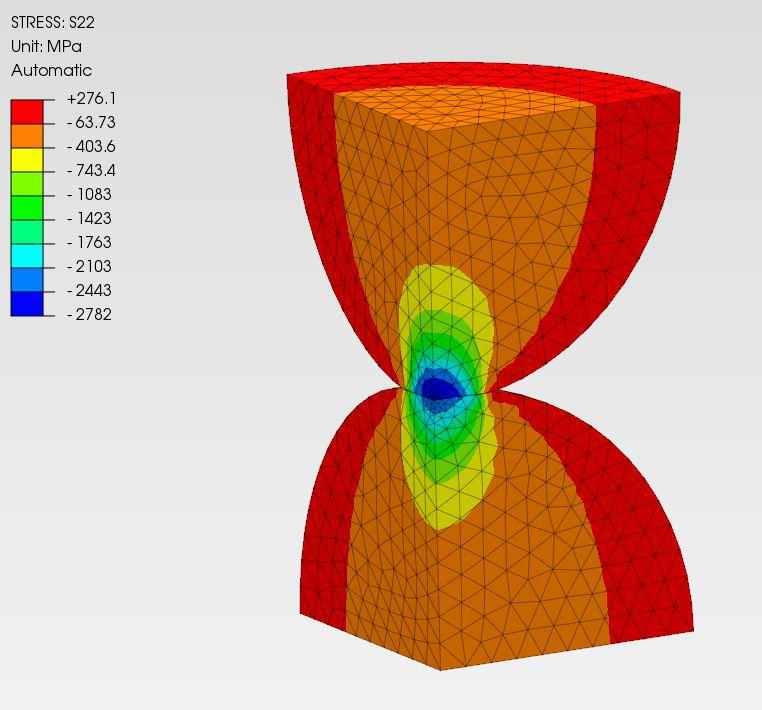
\includegraphics[width=102mm]{fig/08-03.png}
	\caption{2つの球 - 垂直応力}
	\label{fig:08-03}
	\end{figure}
\end{enumerate}